\documentclass{article}
\usepackage[utf8]{inputenc}
\usepackage[spanish]{babel}
\usepackage{graphicx}
\usepackage{listings}
\usepackage{xcolor}

\definecolor{codegreen}{rgb}{0,255,255}
\definecolor{codegray}{rgb}{0.5,0.5,0.5}
\definecolor{codepurple}{rgb}{0.58,0,0.82}
\definecolor{backcolour}{rgb}{0.95,0.95,0.92}

\lstdefinestyle{mystyle}{
    backgroundcolor=\color{backcolour},   
    commentstyle=\color{codegreen},
    keywordstyle=\color{yellow},
    numberstyle=\tiny\color{codegray},
    stringstyle=\color{codegreen},
    basicstyle=\ttfamily\footnotesize,
    breakatwhitespace=false,         
    breaklines=true,                 
    captionpos=b,                    
    keepspaces=true,                 
    numbers=left,                    
    numbersep=5pt,                  
    showspaces=false,                
    showstringspaces=false,
    showtabs=false,                  
    tabsize=2
}
\lstset{style=mystyle}


\title{Informe Parcial II}
\author{daniel.perez19 }
\date{September 2021}

\begin{document}

\begin{titlepage}
    \begin{center}
        \vspace*{1cm}
            
        \Huge
        \textbf{Informe Parcial 2}
            
        \vspace{0.5cm}
        \LARGE
        Informática II
            
        \vspace{1.5cm}
            
        \textbf{Daniel Perez Gallego CC. 1193088770\\Jorge Montaña Cisneros CC.  1007327968}
            
        \vfill
            
        \vspace{0.8cm}
            
        \Large
        Departamento de Ingeniería Electrónica y Telecomunicaciones\\
        Universidad de Antioquia\\
        Medellín\\
        Septiembre de 2021
            
    \end{center}
\end{titlepage}

\tableofcontents
\vspace{1,5cm}
\section{Clases implementadas}

\subsection{Menu}
Clase iteractiva con el usuario, delegada de pedir el nombre de la imagen con su formato, almacenada en la carpeta 'Imagenes'. Retorna la variable 'im', correspondiente a la imagen cargada con el tipo QImage.\\

\subsection{Imagen}
Encargada de manejar la imagen con los parámetros de su alto y ancho, promediar los colores por bloques y crear el .txt generado con el formato adecuado.\\

\subsection{Pixel RGB}
Es la encargada de almacenar los pixeles RGB de la imagen para luego separarlos, tiene como parámetro los colores del RGB\\

\section{Esquema de las clases}
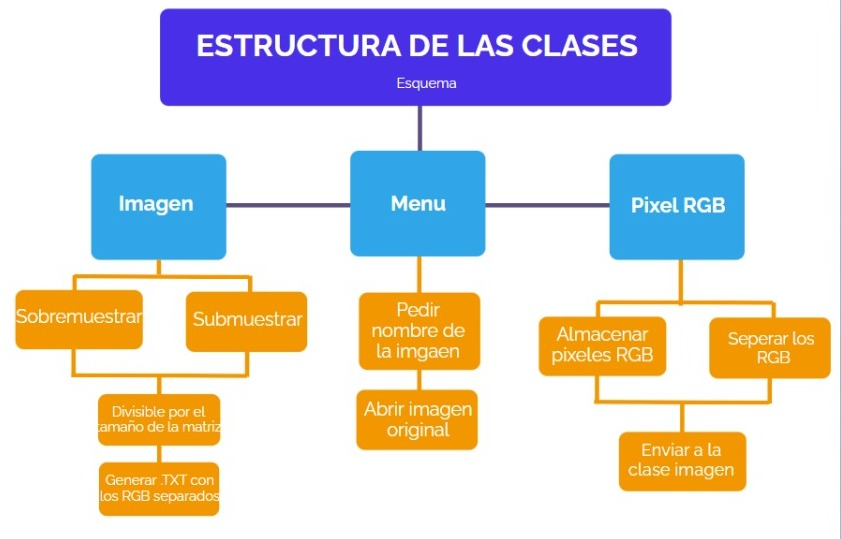
\includegraphics[width=14cm]{Imagenes/clases.jpeg}

\section{Módulos de código de interacción}

\begin{lstlisting}[language=C++, caption=Parámetros de la clase imagen]
class Imagen
{
private:
    int fila, columna;
    vector<vector<Pixel_RGB>> Pixel_color;
public:
    Imagen();
    Imagen(int M, int N);
    void set_color(int x, int y, Pixel_RGB color);  
    int getFila() const;
    void setFila(int value);
    int getColumna() const;
    void setColumna(int value);
    void imprimir_pruebas();
    void txt_generado();
    Pixel_RGB Promedio_Color(int fo, int cantidadF, int co, int cantidadC);
    Pixel_RGB recorrer(int fo, int co);
};
\end{lstlisting}

\newpage
\begin{lstlisting}[language=C++, caption=Clase recorrer]
Pixel_RGB Imagen::recorrer (int fo, int co)
{
    int limF = fo;
    int limC = co;
    int Red = 0, Green= 0, Blue = 0;
    for (int f=fo; f<=limF; f++ ) {
        for (int c=co; c<=limC; c++ ) {
            Red = Pixel_color[f][c].getRed();
            Green = Pixel_color[f][c].getGreen();
            Blue = Pixel_color[f][c].getBlue();
        }
    }

    return Pixel_RGB(Red, Green, Blue);
}
\end{lstlisting}
\vspace{1,5cm}
\begin{lstlisting}[language=C++, caption=Clase promedio color]
Pixel_RGB Imagen::Promedio_Color(int fo, int cantidadF, int co, int cantidadC)
{
    int limF = fo+cantidadF;
    int limC = co+cantidadC;
    int pixeles = cantidadF*cantidadC;
    int sumaRed = 0, sumaGreen= 0, sumaBlue = 0;
    for (int f=fo; f<limF; f++ ) {
        for (int c=co; c<limC; c++ ) {
            sumaRed += Pixel_color[f][c].getRed();
            sumaGreen += Pixel_color[f][c].getGreen();
            sumaBlue += Pixel_color[f][c].getBlue();
        }
    }

    return Pixel_RGB(sumaRed/pixeles, sumaGreen/pixeles, sumaBlue/pixeles);
}
\end{lstlisting}
\vspace{1,5cm}

\begin{lstlisting}[language=C++, caption=Clase set color]
void Imagen::set_color(int x, int y, Pixel_RGB color){
        Pixel_color[x][y].setColor(color);
}
\end{lstlisting}
\section{Estructura del circuito montado}
Para la matriz de LEDs en Tinkerdad, diseñamos un circuito de 16x16 LEDs, hecha con tiras de neopixel. Cada una con su salida conectada a la entrada de la fila/tira superior, la potencia conectada a un sumnistro de energía y todas las coneciones para que el circuito funcione con normalidad\\

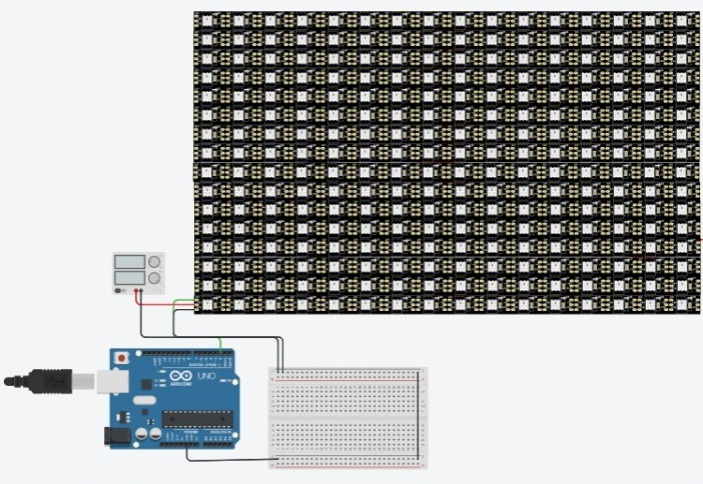
\includegraphics[width=14cm]{Imagenes/circuito.jpeg}

\section{Problemas presentados}
Justo como lo analizamos, el método para reducir y amplificar la imgagen fué la parte más complicada en la implementación, a pesar de que buscamos varias métodos, a la hora de codificarlo se complicaba y comenzamos a buscar un método para simplificarlo, hasta el punto donde consideramos aplicar un nuevo método y empezar casi desde 0.\\

Problemas para la función de sobremuestreo, con los bloques impares.\\

Desconocíamos el formato que debían ser escritos los RGB en el .txt generado para tinkercad y si teníamos que insertar algún método para que el usuario no tenga que copiar y pegar el RGB en el tinkercad\\

La conexión del circuito fué un problema menor gracias a la búsqueda de documentación y videos sobre el código y la conexión en tinkercad; sin embargo, pensábamos que se encenderían los LEDs rápido, pero como no lo hacian debido a toda la información que se procesaba, abortabamos el proceso pensando que el circuito estaba malo, pero no lo estaba, solo éramos muy impacientes. 


\end{document}